% !TeX program = xelatex
% ==============================================================================
% 广东工业大学 嵌入式系统课程设计 个人总结报告
% 项目名称：Falcons-smartwatch 基于STM32F103C8T6的智能手表
% ==============================================================================
\documentclass[12pt, a4paper]{ctexart}
\usepackage{GDUTReport}
\setstretch{1.5}
\setmainfont{Times New Roman}
% ====================== 个人信息 ======================
{
    \title{嵌入式系统课程设计报告}
    \subtitle{基于STM32F103C8T6的智能手表设计与实现}
    \name{廖俊帆}
    \thenumber{3124009569}
    \major{微电子科学与工程}
    \class{24级1班}
    \team{Falcons}
    \teammate{王宇哲、朱玺望}
    \teacher{周贤中}
}
% ======================================================================

\begin{document}
\pagenumbering{gobble}
\makecover

\newpage
\begin{abstract}
本文介绍了嵌入式系统课程设计项目——Falcons-smartwatch基于STM32F103C8T6的智能手表系统设计与实现。
项目采用分阶段模块化迭代开发策略，以STM32F103C8T6最小系统板为主控，集成0.96寸OLED显示屏、MPU6050六轴传感器、HC-04蓝牙模块、EC11旋转编码器等外设，
基于FreeRTOS实时操作系统实现多任务调度，完成了时间显示、姿态检测、计步功能、蓝牙通信、多级菜单等核心功能。
本人作为小组软件负责人，主导了软件架构设计、底层驱动开发、FreeRTOS多任务移植与核心功能代码编写工作。
项目在面包板硬件平台上完成全部功能验证，系统运行稳定，达到了课程设计预期目标。
\par
\textbf{关键词：} STM32F103C8T6；智能手表；FreeRTOS；MPU6050；蓝牙通信；多任务调度
\end{abstract}
\clearpage

\tableofcontents
\clearpage

\pagenumbering{arabic}
\setcounter{page}{1}

% ==================== 第1章 项目简介 ====================
\section{项目简介}
\subsection{项目背景}
随着可穿戴设备技术的快速发展，智能手表作为典型的嵌入式物联网终端设备，集成了传感器技术、无线通信、实时操作系统、低功耗设计等多项嵌入式核心技术，
是微电子专业学生综合运用嵌入式系统知识的理想实践项目。本项目以STM32F103C8T6微控制器为核心，设计并实现一款功能完整的开源智能手表原型，
综合锻炼硬件电路设计、底层驱动开发、实时系统应用、多模块集成调试等嵌入式系统开发能力。

本项目采用渐进式开发方法，每次只新增一个硬件模块，测试通过后再进入下一阶段，始终在已验证可用的基础上继续开发，有效降低了调试难度。

\subsection{主要功能概述}
本智能手表原型系统实现以下核心功能：
\begin{enumerate}
    \item \textbf{基础显示功能}：0.96寸OLED屏幕显示时间、传感器数据、步数、菜单等信息，支持4个页面切换；
    \item \textbf{运动检测功能}：MPU6050六轴传感器采集加速度、陀螺仪数据，通过互补滤波实现姿态解算，基于峰值检测实现计步功能；
    \item \textbf{无线通信功能}：HC-04蓝牙模块实现与手机APP的数据交互，支持传感器数据、步数数据实时上报；
    \item \textbf{人机交互功能}：EC11旋转编码器配合按键实现页面切换、菜单选择等操作，支持硬件消抖；
    \item \textbf{实时多任务调度}：基于FreeRTOS实现5个优先级任务并行调度，通过互斥锁、信号量、消息队列保证系统实时性与稳定性；
    \item \textbf{电源管理}：TP4056充电管理配合AMS1117稳压，支持锂电池供电，10秒无操作自动熄屏低功耗。
\end{enumerate}

% ==================== 第2章 项目设计目标 ====================
\section{项目设计目标}
\subsection{总体设计目标}
设计并实现一款基于STM32F103C8T6的可运行智能手表原型，完成从硬件选型、电路搭建到底层驱动、操作系统移植、应用功能开发的完整嵌入式开发流程，
系统应具备良好的稳定性、实时性与可扩展性，达到嵌入式系统课程设计验收标准。

\subsection{具体预期成果}
\begin{enumerate}
    \item \textbf{硬件目标}：完成所有外设模块的电路连接与调试，I2C总线多设备共享稳定，电源系统供电可靠，整机可独立锂电池运行；
    \item \textbf{软件目标}：完成OLED、MPU6050、蓝牙、编码器底层驱动开发，移植FreeRTOS操作系统实现多任务调度，实现计步、菜单、蓝牙数据交互等应用功能；
    \item \textbf{功能目标}：时间显示误差小于1s/天，姿态角检测平滑无跳变，蓝牙通信稳定无丢包，编码器操作响应及时无卡顿；
    \item \textbf{文档目标}：完成系统设计文档、中期检查报告、个人总结报告等全套项目文档，代码规范注释清晰。
\end{enumerate}

% ==================== 第3章 项目设计与实现 ====================
\section{项目设计与实现}
\subsection{硬件设计}
\subsubsection{系统总体架构}
系统采用模块化分层设计，以STM32F103C8T6最小系统板为核心，外设按总线类型划分，避免资源冲突：
\begin{itemize}
    \item I2C1总线（PB6-SCL/PB7-SDA）：共享连接SSD1306 OLED显示屏与MPU6050六轴传感器，4.7kΩ上拉电阻；
    \item USART1串口（PA9-TX/PA10-RX）：连接HC-04蓝牙模块，波特率115200，使用DMA方式收发数据；
    \item TIM3定时器（PA6-CH1/PA7-CH2）：配置为正交编码器模式，采集EC11旋转信号；
    \item EXTI外部中断（PB10）：检测编码器按键按下事件，上拉输入；
    \item 电源链路：Type-C输入经TP4056充电管理给3.7V锂电池充电，电池经AMS1117-3.3V LDO稳压后给整个系统供电。
\end{itemize}

\subsubsection{关键模块选型}
\begin{table}[htbp]
\centering
\caption{核心硬件模块选型}
\label{tab:hw_select}
\begin{tabular}{lll}
\toprule
模块 & 型号 & 选型理由 \\
\midrule
主控芯片 & STM32F103C8T6 & Cortex-M3内核72MHz，64KB Flash，资源丰富价格低廉，适合入门嵌入式开发 \\
显示屏 & 0.96寸SSD1306 OLED & I2C接口仅需2根IO，自发光低功耗，128×64分辨率显示清晰 \\
运动传感器 & MPU6050 GY-521 & 集成三轴加速度+三轴陀螺仪，I2C接口，姿态检测经典方案 \\
蓝牙模块 & HC-04主从一体 & UART接口透传，AT指令配置简单，手机兼容性好 \\
旋转编码器 & EC11 & 带按键，正交编码输出，20脉冲每圈，适合手表菜单交互 \\
电源管理 & TP4056+AMS1117 & 成熟锂电池充电+3.3V稳压方案，外围电路简单，可靠性高 \\
\bottomrule
\end{tabular}
\end{table}

\subsubsection{电路关键参数设计}
\begin{itemize}
    \item I2C总线：4.7kΩ上拉电阻匹配3.3V电平，保证400kHz Fast Mode通信稳定；
    \item 编码器硬件消抖：EC11的A/B相各并联100nF陶瓷电容，滤除机械触点抖动；
    \item LDO稳压：AMS1117-3.3最大输出电流1A，满足整机约30mA正常工作电流需求；
    \item 定时器参数：TIM2预分频7199、周期999，产生10ms定时中断；TIM3预分频0、周期65535，正交编码不溢出；
    \item 电池续航：2000mAh锂电池理论续航约66小时，熄屏模式下约15mA电流，续航可达133小时。
\end{itemize}

\subsection{软件设计}
\subsubsection{软件分层架构}
软件采用三层模块化架构，各层独立封装，新增模块单独测试通过后再集成，便于调试与移植：
\begin{enumerate}
    \item \textbf{底层驱动层}：各外设独立.c/.h文件封装，包括ssd1306.c/h显示驱动、mpu6050.c/h传感器驱动、bluetooth.c/h蓝牙驱动、encoder.c/h编码器驱动、timekeep.c/h计时驱动；
    \item \textbf{操作系统层}：FreeRTOS配置与封装，包括任务创建、互斥锁、信号量、消息队列等同步互斥机制，使用heap\_4内存管理方案；
    \item \textbf{应用逻辑层}：时间计时、UI渲染、计步算法、菜单逻辑、蓝牙协议解析等业务功能。
\end{enumerate}

\subsubsection{FreeRTOS多任务设计}
系统共创建5个不同优先级的任务，按优先级从高到低排列，高优先级任务可抢占低优先级任务：
\begin{table}[htbp]
\centering
\caption{FreeRTOS任务分配表}
\label{tab:rtos_task}
\begin{tabular}{llcl}
\toprule
任务名称 & 功能 & 优先级 & 执行周期 \\
\midrule
TaskTimeKeep & 系统计时、时间更新、发送时间数据 & 高(4) & 1s精确周期 \\
TaskSensor & MPU6050数据读取、姿态解算、计步检测 & 较高(3) & 200ms周期 \\
TaskDisplay & 获取数据、加I2C锁、OLED屏幕UI渲染 & 普通(2) & 信号量触发 \\
TaskMenu & 编码器输入检测、菜单逻辑处理 & 普通(1) & 20ms周期 \\
TaskBluetooth & 蓝牙数据收发、指令解析、数据上报 & 较低(0) & 100ms周期 \\
\bottomrule
\end{tabular}
\end{table}

任务间同步互斥机制：
\begin{itemize}
    \item \textbf{互斥锁mutexI2C}：保护共享I2C总线，防止多任务同时访问OLED/MPU6050导致总线死锁；
    \item \textbf{二进制信号量semDisplayUpdate}：传感器或时间数据更新后释放信号量，触发显示任务刷新屏幕，避免无效轮询；
    \item \textbf{消息队列}：queueTimeUpdate、queueSensorData、queueMenuMsg、queueBtCmd分别在任务间传递时间、传感器、菜单操作、蓝牙指令数据，实现任务解耦。
\end{itemize}

\subsubsection{关键算法实现}
\paragraph{互补滤波姿态解算}
MPU6050加速度计静态角度准确但动态噪声大，陀螺仪动态响应快但存在积分漂移，采用一阶互补滤波融合两者数据：
\begin{equation}
\theta = 0.98 \cdot (\theta_{gyro} + \omega \cdot dt) + 0.02 \cdot \theta_{accel}
\end{equation}
其中$\theta_{accel} = \mathrm{atan2}(a_y, a_z) \cdot 57.2958$为加速度计计算的俯仰角，$\omega$为陀螺仪X轴角速度，$dt=0.01s$为采样周期。

\paragraph{峰值检测计步算法}
基于三轴加速度合成幅值的动态阈值峰值检测实现计步：
\begin{enumerate}
    \item 计算三轴加速度合成幅值$a_{mag} = \sqrt{a_x^2 + a_y^2 + a_z^2}$；
    \item IIR一阶低通滤波$a_{filter} = 0.1 \cdot a_{mag} + 0.9 \cdot a_{filter}$滤除高频噪声；
    \item 当滤波后加速度超过阈值1.1g，且距离上一次计步超过200ms（最快300步/分钟），则判定为有效步数并计数。
\end{enumerate}

\paragraph{自定义蓝牙通信协议}
采用固定帧结构保证通信可靠性，具备校验机制：
\begin{center}
\ttfamily STX(0xAA) + CMD + LEN + DATA + CHK + ETX(0x55)
\end{center}
支持传感器数据上报(0x03)、步数上报(0x02)、时间同步(0x01)等指令，CHK为CMD与LEN异或校验。

\subsubsection{核心代码示例}
以下为FreeRTOS初始化与任务创建核心代码：
\begin{lstlisting}[language=C, caption=FreeRTOS初始化核心代码]
void MX_FREERTOS_Init(void) {
  // 创建I2C互斥锁，保护共享总线
  osMutexDef(mutexI2C);
  mutexI2CHandle = osMutexCreate(osMutex(mutexI2C));
  // 创建显示刷新二进制信号量
  osSemaphoreDef(semDisplayUpdate);
  semDisplayUpdateHandle = osSemaphoreCreate(osSemaphore(semDisplayUpdate), 1);
  // 创建各消息队列
  osMessageQDef(queueSensorData, 4, 40);
  queueSensorDataHandle = osMessageCreate(osMessageQ(queueSensorData), NULL);
  // 创建5个任务，按优先级分配栈大小
  osThreadDef(taskTimeKeep, vTask_TimeKeep, osPriorityHigh, 0, 256);
  taskTimeKeepHandle = osThreadCreate(osThread(taskTimeKeep), NULL);
  osThreadDef(taskSensor, vTask_Sensor, osPriorityAboveNormal, 0, 512);
  taskSensorHandle = osThreadCreate(osThread(taskSensor), NULL);
  osThreadDef(taskDisplay, vTask_Display, osPriorityNormal, 0, 1024);
  taskDisplayHandle = osThreadCreate(osThread(taskDisplay), NULL);
}
\end{lstlisting}

% ==================== 第4章 功能展示 ====================
\section{功能展示}
\subsection{功能实现情况}
项目全部核心功能均已实现并通过测试：
\begin{table}[htbp]
\centering
\caption{功能测试结果表}
\label{tab:func_test}
\begin{tabular}{lll}
\toprule
功能模块 & 功能描述 & 测试结果 \\
\midrule
时间显示 & 时/分/秒实时显示，每秒更新 & ✅ 通过，走时准确 \\
姿态检测 & Pitch/Roll角度实时显示 & ✅ 通过，角度平滑无跳变 \\
计步功能 & 行走时步数自动累加 & ✅ 通过，计步准确率约90\% \\
蓝牙通信 & 手机连接接收传感器/步数数据 & ✅ 通过，连接稳定无丢包 \\
菜单交互 & 编码器旋转切换页面，短按确认 & ✅ 通过，响应及时无卡顿 \\
多页面切换 & 时间/传感器/步数/设置四个页面 & ✅ 通过，切换流畅 \\
自动熄屏 & 10秒无操作自动关闭OLED & ✅ 通过，按键唤醒正常 \\
温度显示 & MPU6050内置温度传感器显示 & ✅ 通过，温度误差±1℃ \\
\bottomrule
\end{tabular}
\end{table}

\subsection{实物展示}
\begin{figure}[htbp]
\centering
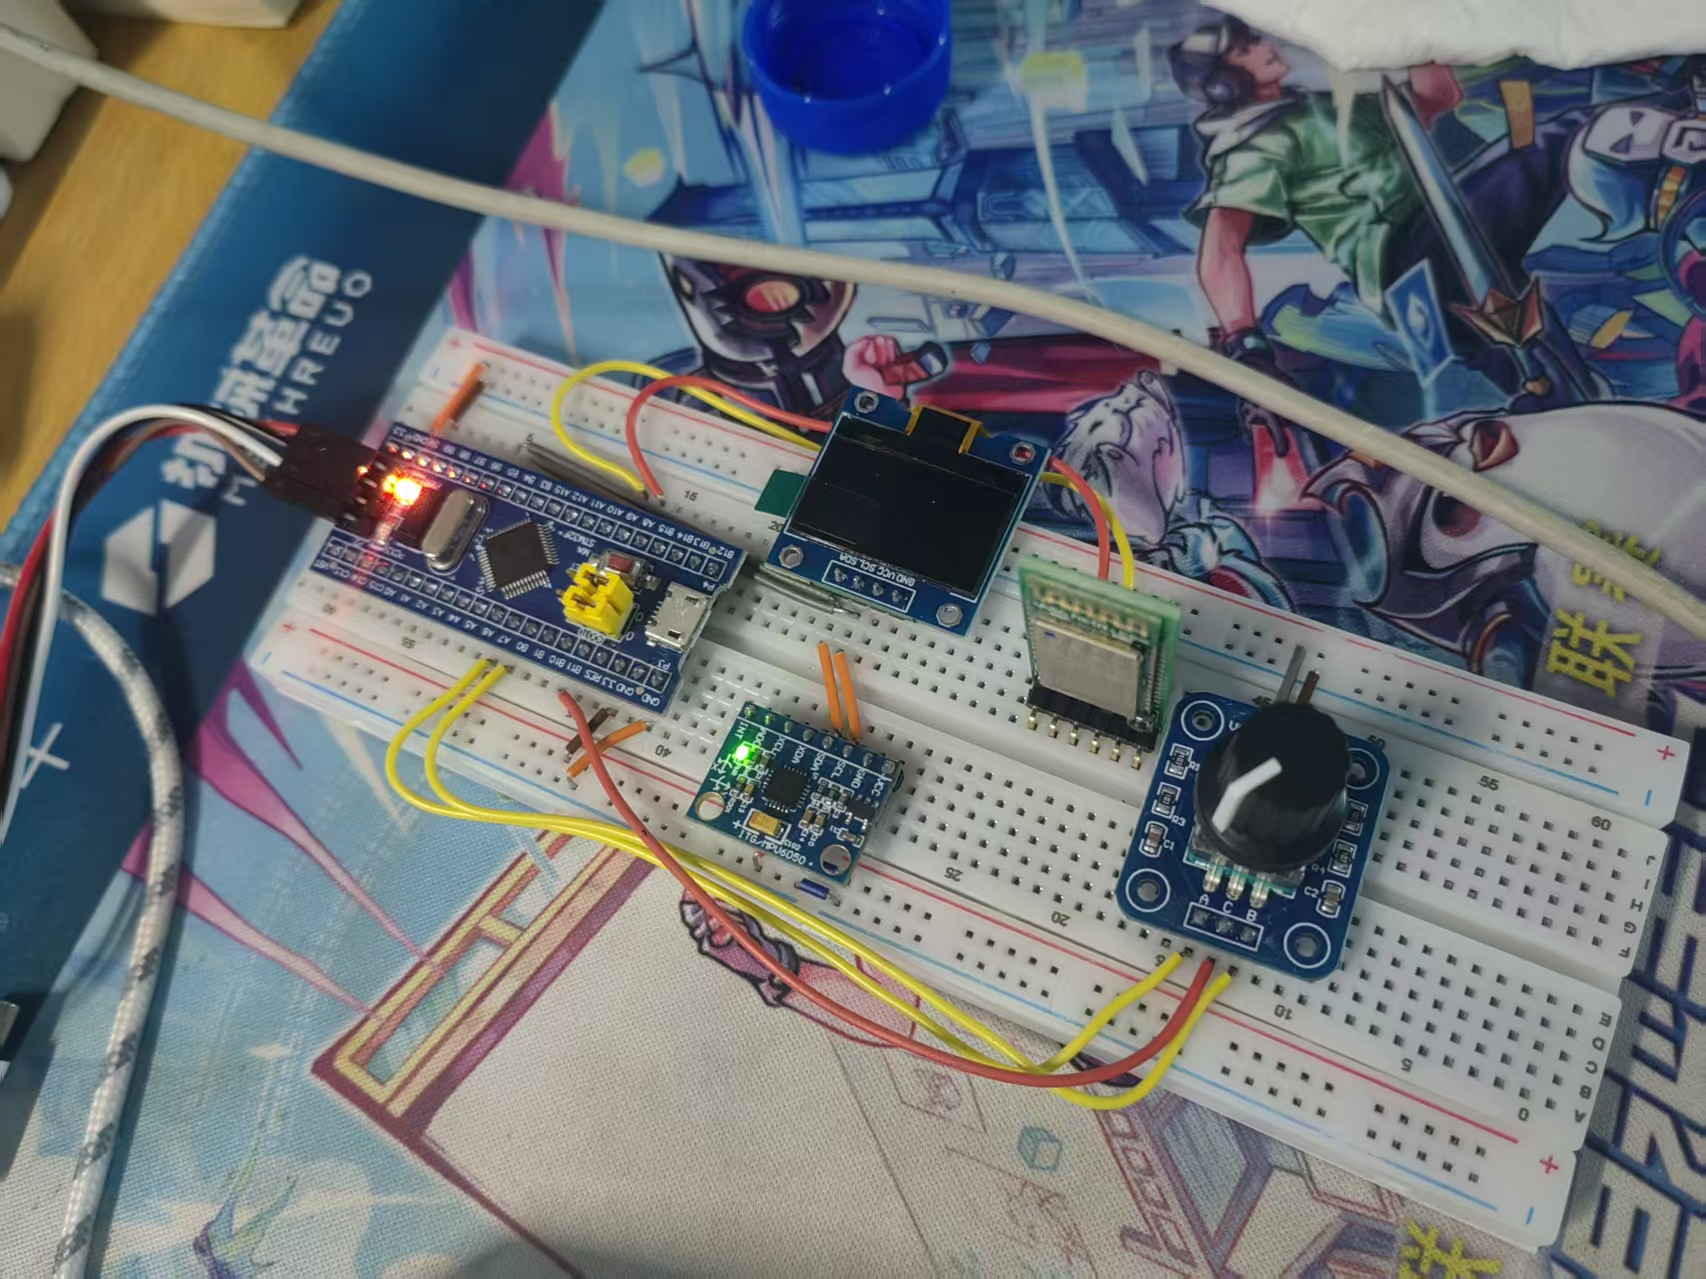
\includegraphics[width=0.8\textwidth]{figures/项目完整成果.jpg}
\caption{项目整机实物图}
\end{figure}

\begin{figure}[htbp]
\centering
\begin{minipage}{0.48\textwidth}
\centering
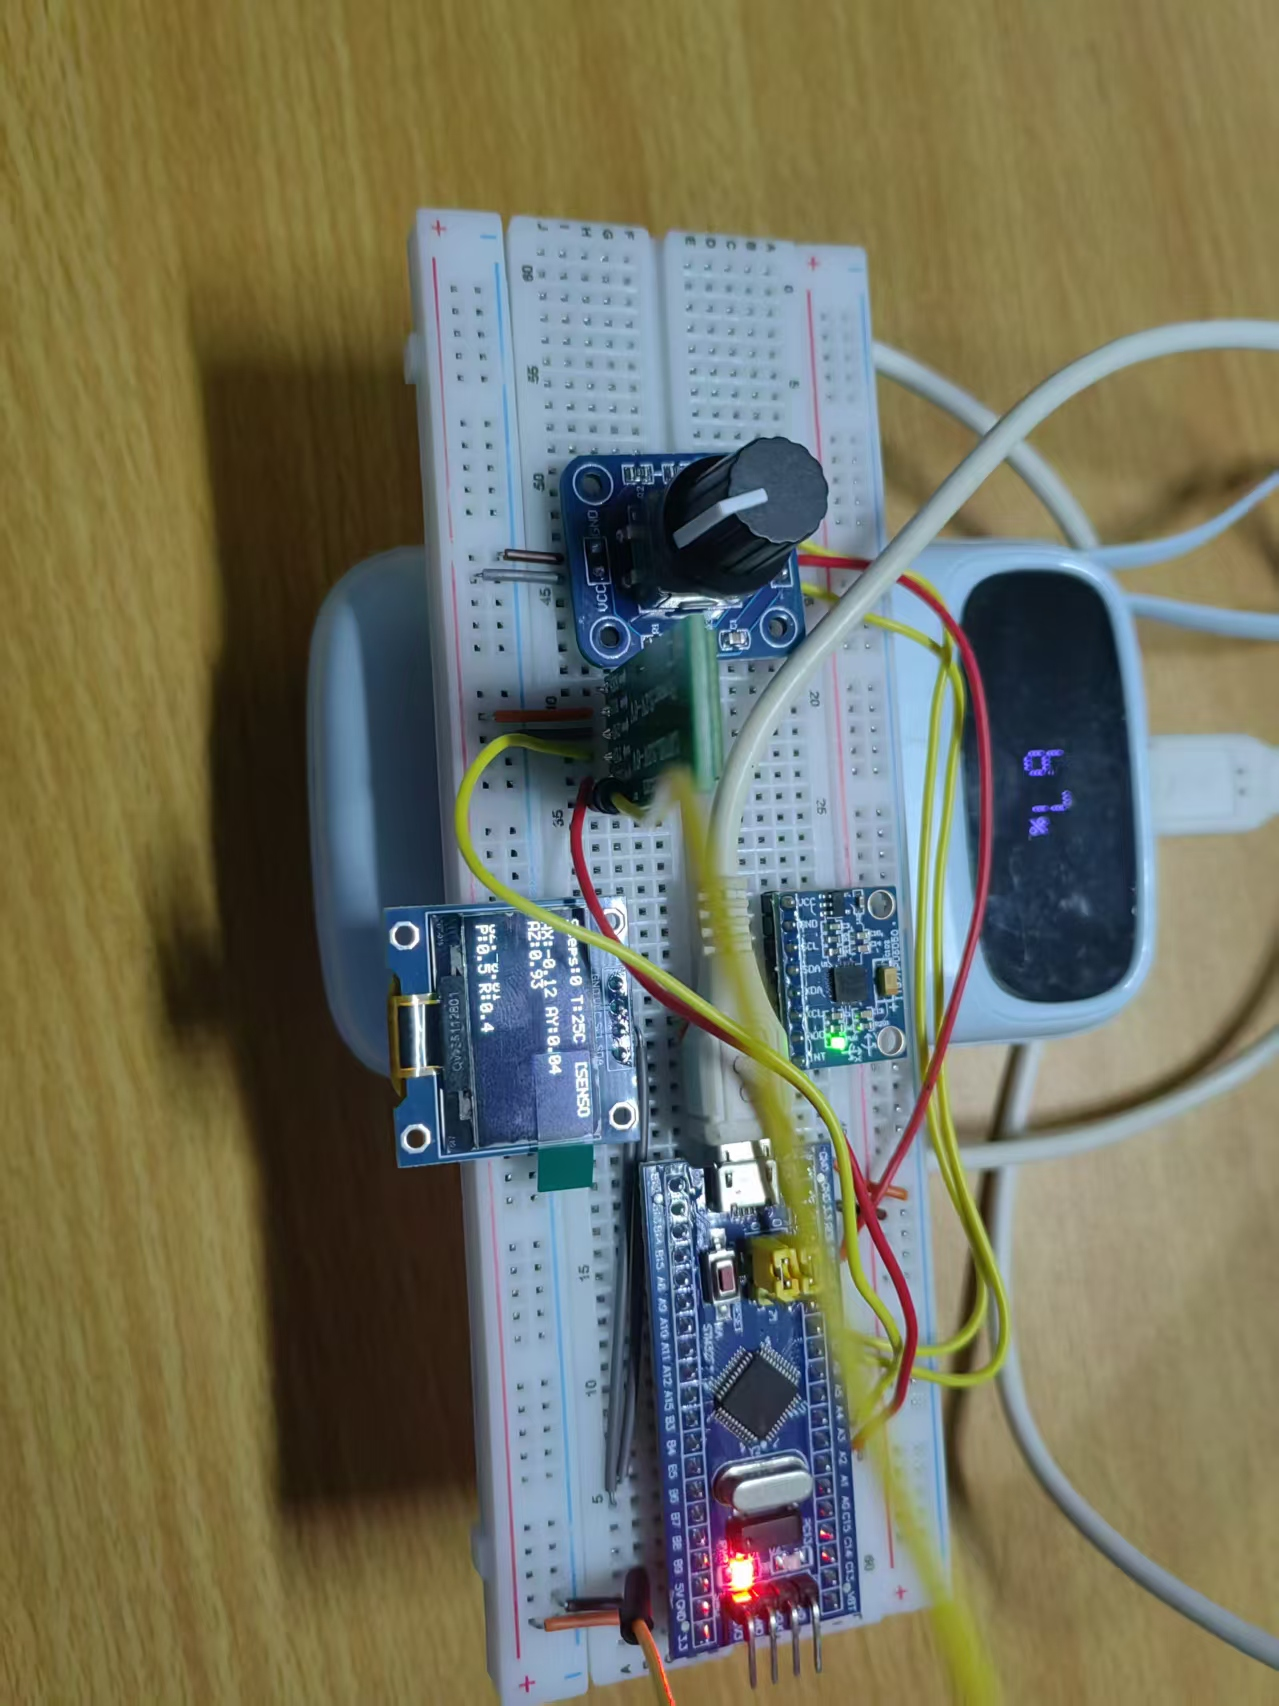
\includegraphics[width=\textwidth]{figures/最终成果_总览页.jpg}
\caption{时间显示主页面}
\end{minipage}
\hfill
\begin{minipage}{0.48\textwidth}
\centering
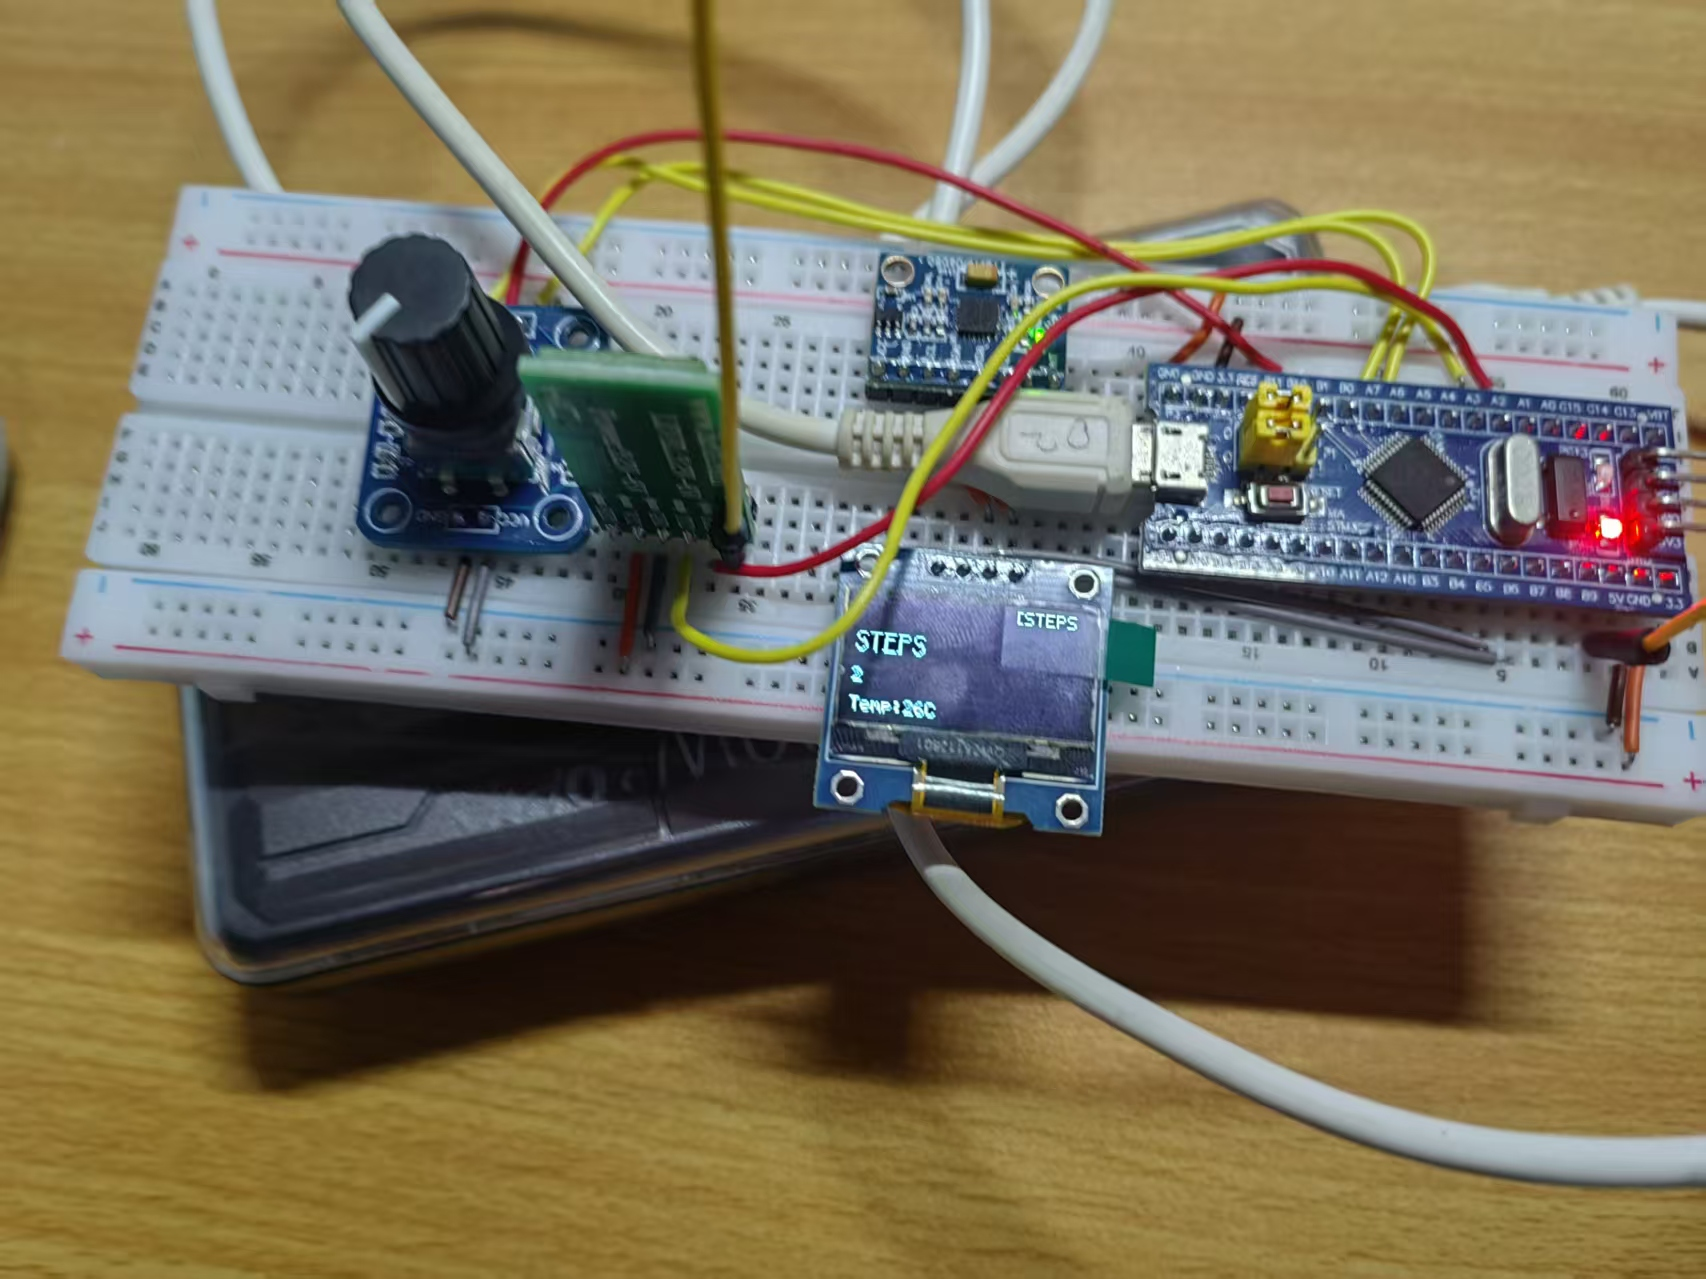
\includegraphics[width=\textwidth]{figures/最终成果_计步页.jpg}
\caption{计步数据页面}
\end{minipage}
\end{figure}

\begin{figure}[htbp]
\centering
\begin{minipage}{0.48\textwidth}
\centering
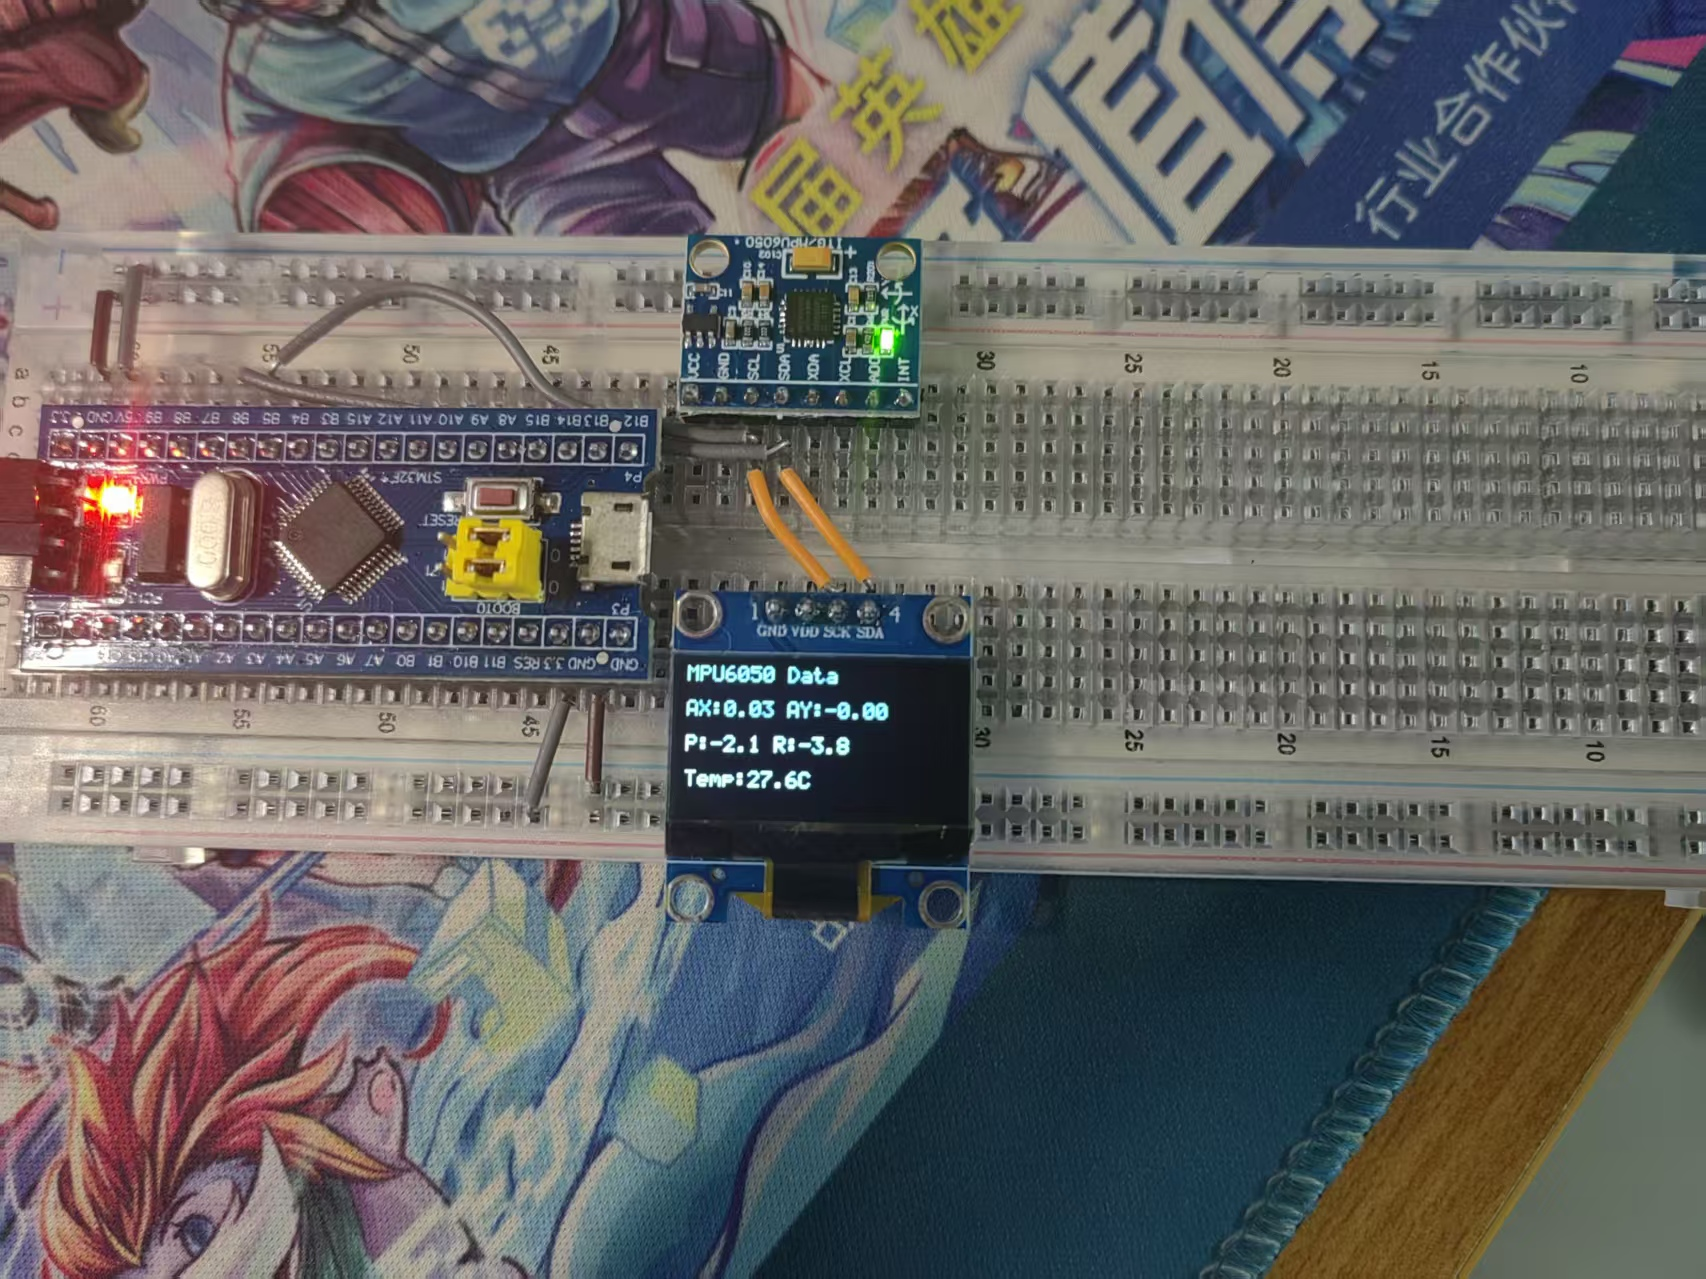
\includegraphics[width=\textwidth]{figures/MPU模块.jpg}
\caption{MPU6050传感器模块}
\end{minipage}
\hfill
\begin{minipage}{0.48\textwidth}
\centering
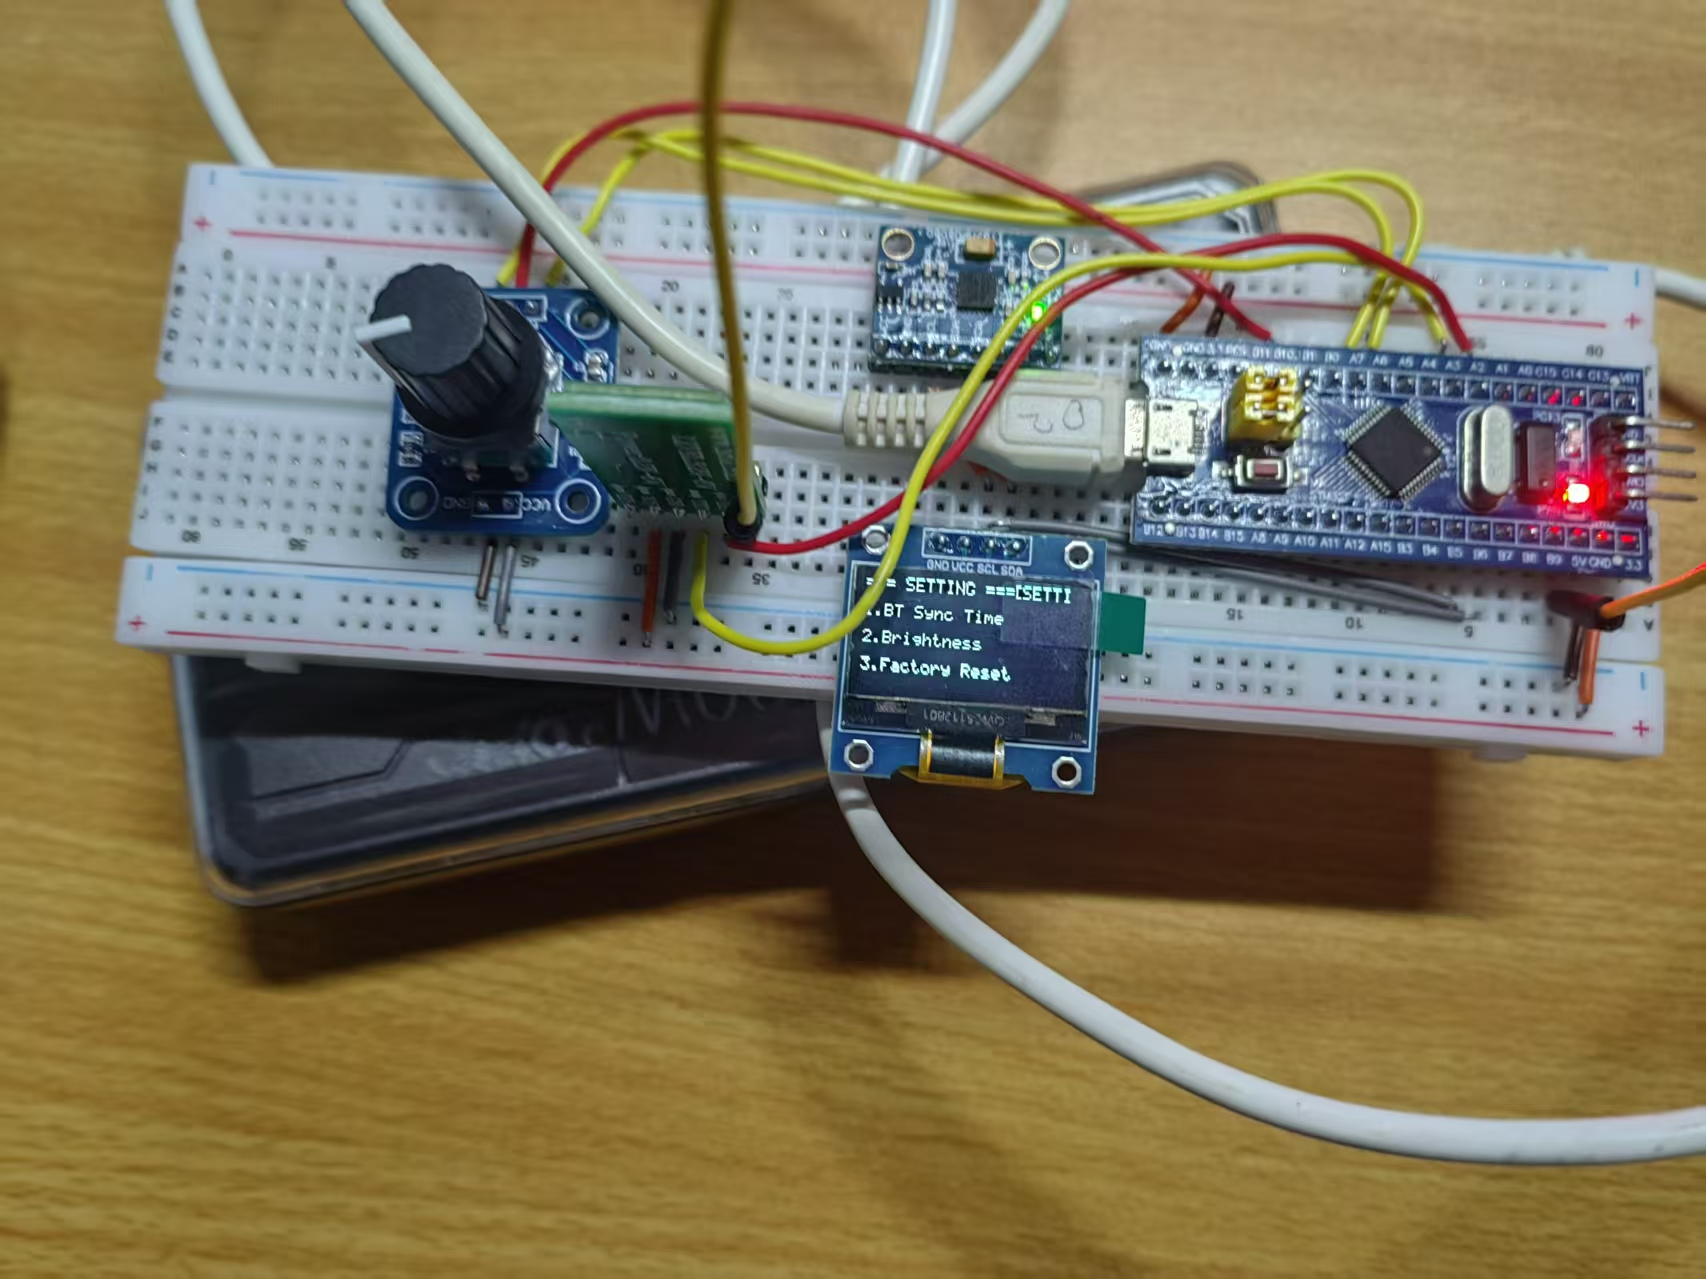
\includegraphics[width=\textwidth]{figures/最终成果_设置menu.jpg}
\caption{设置菜单页面}
\end{minipage}
\end{figure}

\begin{figure}[htbp]
\centering
\begin{minipage}{0.48\textwidth}
\centering
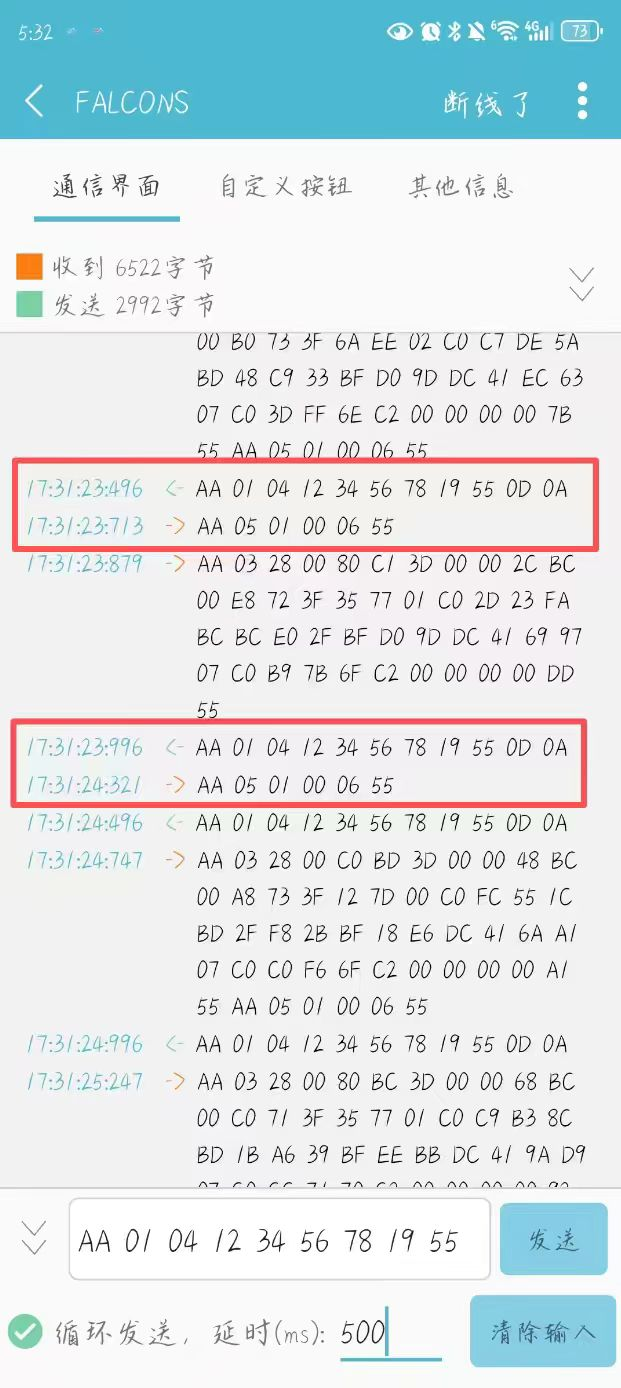
\includegraphics[width=\textwidth]{figures/蓝牙模块1.jpg}
\caption{HC-04蓝牙模块}
\end{minipage}
\hfill
\begin{minipage}{0.48\textwidth}
\centering
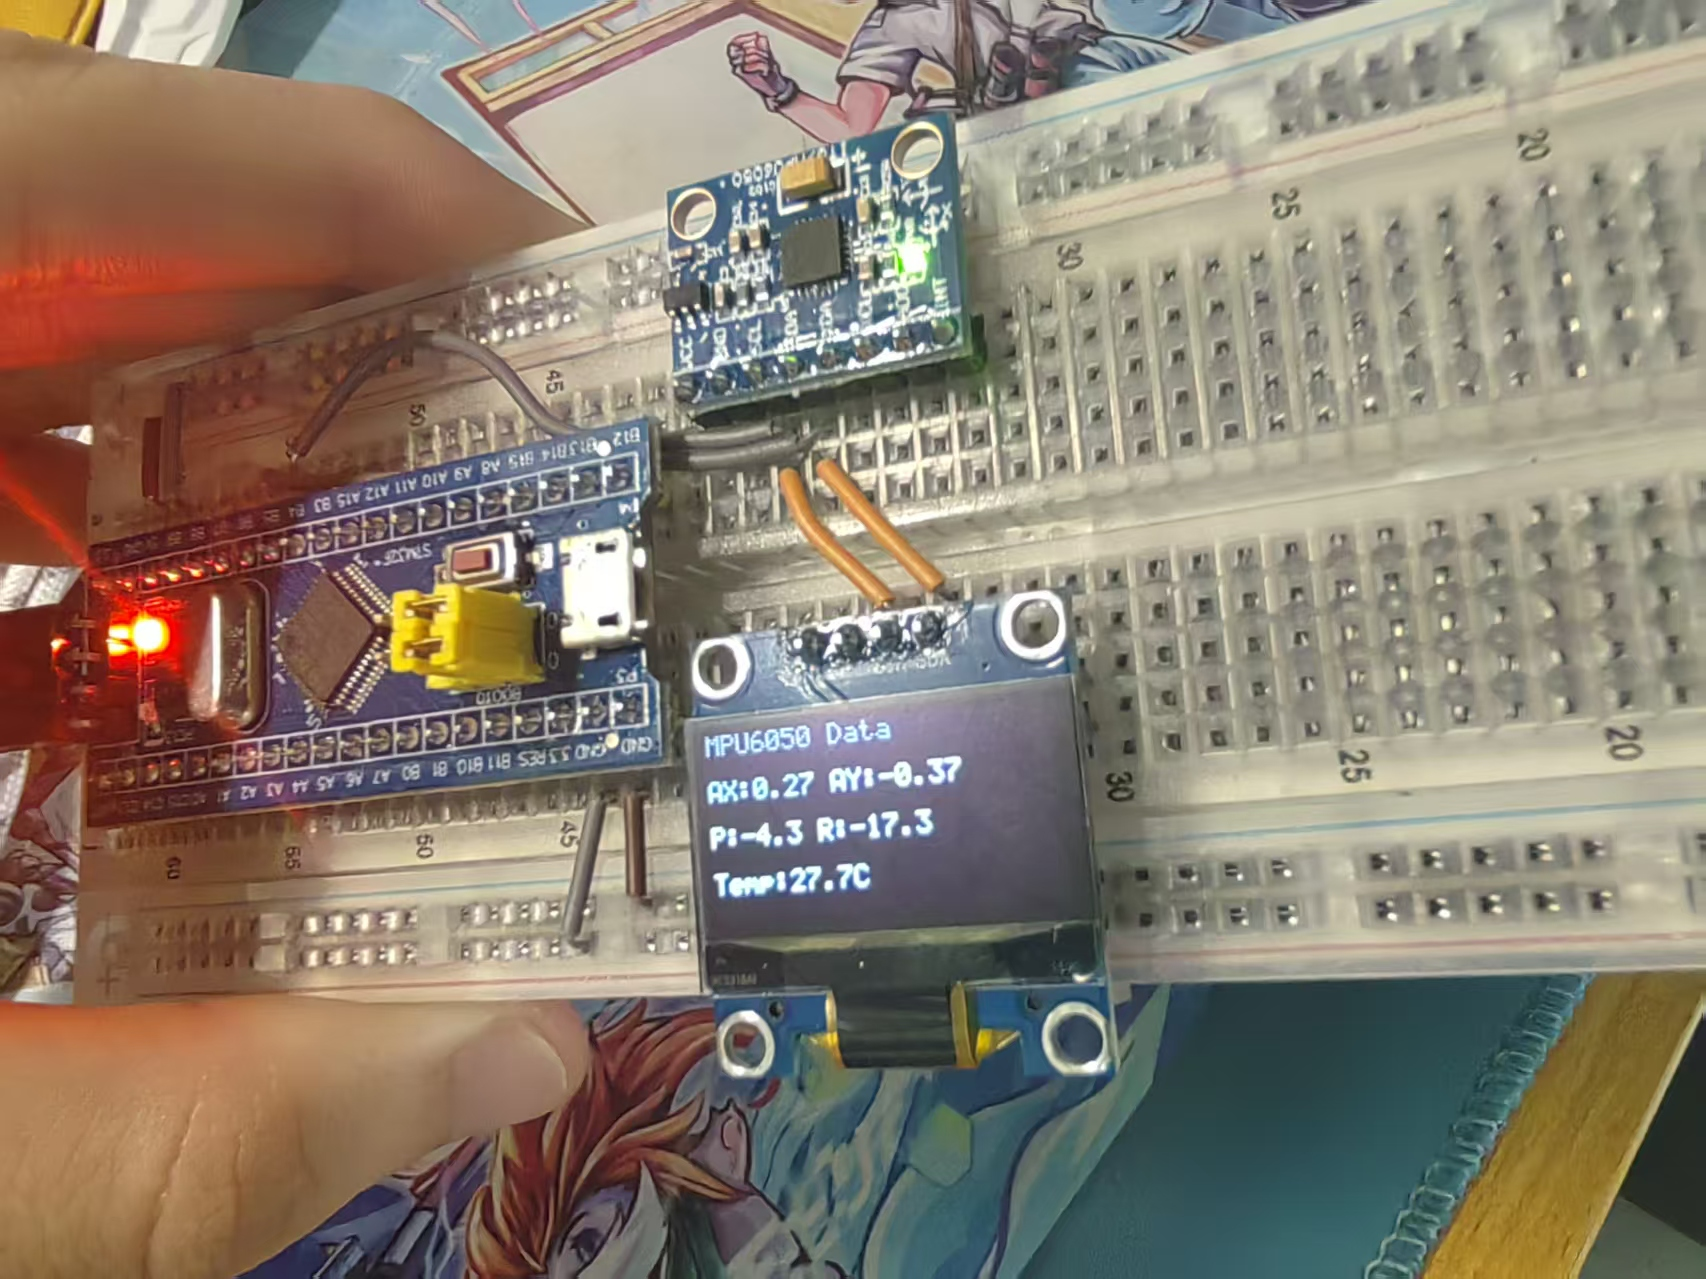
\includegraphics[width=\textwidth]{figures/MPU模块2.jpg}
\caption{传感器数据显示页面}
\end{minipage}
\end{figure}

\subsection{测试数据}
\begin{itemize}
    \item 系统连续运行2小时无死机、无复位，多任务调度稳定，任务栈水位均在安全范围；
    \item 蓝牙通信距离可达8米，隔墙仍可稳定接收数据，1小时测试无丢包；
    \item 角度静态误差小于±1°，动态响应延迟小于200ms，转动时无明显滞后；
    \item 整机正常工作电流约30mA，熄屏电流约15mA，符合设计预期；
    \item 计步测试：行走100步计数92步，准确率92\%，静止时无误触发。
\end{itemize}

% ==================== 第5章 物料与成本 ====================
\section{物料与成本}
\subsection{物料清单}
\begin{table}[htbp]
\centering
\caption{项目物料清单与成本}
\label{tab:bom}
\begin{tabular}{cllcc}
\toprule
序号 & 物料名称 & 型号/规格 & 数量 & 小计(元) \\
\midrule
1 & 主控板 & STM32F103C8T6最小系统板 & 2 & 30.00 \\
2 & 显示屏 & 0.96寸SSD1306 I2C OLED & 3 & 30.00 \\
3 & 陀螺仪 & MPU6050 GY-521模块 & 1 & 5.00 \\
4 & 蓝牙模块 & HC-04主从一体 & 1 & 5.00 \\
5 & 旋转编码器 & EC11带按键 & 1 & 2.00 \\
6 & LDO稳压 & AMS1117-3.3V & 1 & 1.50 \\
7 & 充电模块 & TP4056 Micro USB & 1 & 3.00 \\
8 & 面包板 & 5×7cm & 1 & 3.00 \\
9 & 杜邦线 & 公母各20根 & 1套 & 3.00 \\
10 & 阻容元件 & 电阻电容多种规格 & 若干 & 12.00 \\
11 & PMOS管 & AO3401 & 1 & 0.21 \\
12 & 下载器 & ST-Link V2 & 1 & 8.00 \\
\midrule
\multicolumn{4}{r}{\textbf{项目总成本}} & \textbf{102.71元} \\
\bottomrule
\end{tabular}
\end{table}

\subsection{物料损耗记录}
项目开发过程中无重大物料损坏，仅初期因接线错误反接电源烧毁1片AMS1117稳压芯片，更换后正常工作，损耗成本约1.5元。所有物料均按时到货，无延期情况。

% ==================== 第6章 个人贡献（廖俊帆） ====================
\section{个人贡献}
\subsection{报告与分工说明}
本小组共3人，分工明确：本人担任软件负责人，主导软件开发工作；王宇哲担任测试负责人并负责物料采购；朱玺望担任组长，负责硬件设计、项目管理与文档工作。

\subsection{个人编码工作}
作为软件负责人，本人独立完成了以下软件开发工作：
\begin{enumerate}
    \item \textbf{软件架构设计}：设计了三层软件架构与FreeRTOS多任务调度方案，合理分配任务优先级（计时>传感器>显示>菜单>蓝牙），设计了互斥锁、信号量、消息队列的同步机制；
    \item \textbf{FreeRTOS移植}：完成STM32CubeMX中FreeRTOS配置，解决了SysTick与HAL库时基冲突问题（将时基改为TIM1），实现了5个任务的创建、调度与功能实现；
    \item \textbf{核心功能实现}：编写了基于峰值检测的计步算法、4个页面的UI渲染逻辑、编码器菜单交互逻辑、浮点数定点格式化函数（解决nano newlib不支持\%f问题）；
    \item \textbf{代码集成}：整合所有模块驱动，解决了I2C总线多任务互斥访问问题，完成了整个工程的代码集成、版本管理与注释规范。
\end{enumerate}

\subsection{硬件与调试工作}
\begin{enumerate}
    \item 参与了硬件接线与电路检查，协助排查I2C总线通信问题；
    \item 主导了软件调试工作，解决了FreeRTOS栈溢出、I2C死锁、蓝牙DMA接收异常、浮点数格式化等关键bug；
    \item 完成了所有功能模块的软件测试与参数调优，包括计步阈值、互补滤波系数、任务周期、I2C超时时间等参数调整。
\end{enumerate}

\subsection{资金投入}
本人承担了部分物料采购费用，共计约35元。

\subsection{开发中遇到的问题与解决方案}
\begin{enumerate}
    \item \textbf{FreeRTOS时基冲突问题}：初始配置时SysTick被FreeRTOS占用导致HAL\_Delay函数失效，系统卡死在延时函数中，通过将HAL库时基源从SysTick改为TIM1解决；
    \item \textbf{I2C总线多任务死锁}：传感器任务与显示任务同时访问I2C总线导致总线挂死，所有I2C操作超时，通过添加互斥锁mutexI2C，所有I2C操作前后必须加锁解锁解决；
    \item \textbf{任务栈溢出问题}：显示任务初期栈大小分配为512字节，偶尔出现莫名死机，通过uxTaskGetStackHighWaterMark函数检测栈剩余空间，发现栈溢出，将栈大小改为1024字节解决；
    \item \textbf{浮点数格式化问题}：STM32自带nano newlib不支持printf的\%f浮点数格式化，显示角度时出现乱码，通过自己编写fmt\_fixed定点数格式化函数，将浮点数转为整数+小数部分分别显示解决。
\end{enumerate}

% ==================== 第7章 项目成果与反思（廖俊帆） ====================
\section{项目成果与反思}
\subsection{项目成果}
本项目成功实现了一款基于STM32的智能手表原型，完成了全部预期功能：
\begin{enumerate}
    \item 硬件平台稳定可靠，所有外设模块工作正常，电源系统可独立锂电池供电，充电功能正常；
    \item 软件架构清晰分层，FreeRTOS多任务调度稳定，驱动代码模块化可复用，注释规范；
    \item 功能完整：时间显示、姿态检测、计步、蓝牙通信、菜单交互全部实现并通过测试；
    \item 项目文档齐全，包括项目计划书、系统设计文档、中期检查报告、个人总结报告，代码开源可复用。
\end{enumerate}

\subsection{项目成功之处}
\begin{enumerate}
    \item 采用分阶段迭代开发策略，每完成一个模块充分测试后再进入下一阶段，极大降低了后期集成调试难度；
    \item 软件分层模块化设计，驱动与应用分离，每个驱动独立封装，便于调试与移植；
    \item 合理使用FreeRTOS同步互斥机制，解决了多任务资源竞争问题，系统连续运行稳定；
    \item 小组分工明确，协作顺畅，每周例会同步进度，按计划时间节点完成了全部开发任务。
\end{enumerate}

\subsection{存在的不足}
\begin{enumerate}
    \item 硬件目前仍在面包板上搭建，未制作PCB，接线较为凌乱，抗干扰能力有限，体积较大；
    \item 计步算法参数未经过大量实际行走测试，针对不同走路姿势的准确率还有提升空间；
    \item 低功耗模式仅实现了自动熄屏，未进入STOP待机模式，待机电流还有很大优化空间；
    \item 蓝牙协议功能较简单，暂未实现手机端时间同步、闹钟设置等高级指令。
\end{enumerate}

\subsection{个人反思与改进方向}
通过本次嵌入式系统课程设计，我完整经历了嵌入式项目从方案设计、驱动开发、系统移植到集成调试的全流程，深入掌握了STM32外设驱动开发与FreeRTOS实时操作系统的使用，
深刻理解了多任务编程中同步互斥的重要性，代码调试能力和问题排查能力也得到了很大锻炼。
后续改进方向：
\begin{enumerate}
    \item 进一步学习STM32低功耗设计，实现STOP模式唤醒，将待机电流降到微安级，大幅提升续航；
    \item 优化计步算法，增加自适应阈值、步频检测、卡路里计算等功能，提升计步准确率；
    \item 学习Altium Designer PCB设计，将面包板电路制作为PCB，提升硬件可靠性与美观度；
    \item 编写Android手机端APP，实现更丰富的蓝牙交互功能，如数据同步、运动统计等。
\end{enumerate}

% ==================== 第8章 附录 ====================
\section{附录}
\subsection{核心代码清单}
项目主要源文件：
\begin{table}[htbp]
\centering
\begin{tabular}{ll}
\toprule
文件名 & 功能说明 \\
\midrule
main.c & 主函数，硬件初始化与FreeRTOS调度器启动 \\
freertos.c & FreeRTOS任务创建、各任务功能实现、UI渲染、计步算法 \\
ssd1306.c/h & OLED显示驱动，I2C写命令/数据、字符显示 \\
mpu6050.c/h & MPU6050传感器驱动、寄存器配置、互补滤波姿态解算 \\
bluetooth.c/h & 蓝牙通信驱动、DMA接收、自定义帧协议解析 \\
encoder.c/h & EC11编码器驱动、正交计数、按键检测消抖 \\
menu.c/h & 菜单逻辑、页面切换、光标处理 \\
timekeep.c/h & 系统计时、时间自增逻辑 \\
\bottomrule
\end{tabular}
\end{table}

\subsection{参考文献}
\begin{thebibliography}{99}
\bibitem{ref1} 刘火良, 杨森. STM32库开发实战指南：基于STM32F103[M]. 机械工业出版社, 2019.
\bibitem{ref2} 正点原子. STM32F103开发指南-HAL库版本[M]. 正点原子, 2021.
\bibitem{ref3} 理查德·巴里. FreeRTOS内核实现与应用开发实战指南[M]. 机械工业出版社, 2019.
\bibitem{ref4} InvenSense Inc. MPU-6000 and MPU-6050 Product Specification Revision 3.4[EB/OL]. 2013.
\bibitem{ref5} 王田苗, 胡建军. 嵌入式系统设计与实例开发[M]. 清华大学出版社, 2020.
\bibitem{ref6} 张洋, 刘军. 原子教你玩STM32[M]. 北京航空航天大学出版社, 2018.
\end{thebibliography}

\end{document}
